\documentclass[letterpaper,12pt, twoside]{book}

\usepackage[letterpaper, inner=2cm,outer=1.5cm, bottom = 2cm, top = 2.5cm]{geometry}
\usepackage{import}
\usepackage{preamble}
\usepackage{pdfpages}
\usepackage{makeidx}
    \makeindex
%\usepackage{mathpazo}

% \geometry{ }
    
\input GoudyIn.fd
\newcommand*\initfamily{\usefont{U}{GoudyIn}{xl}{n}}
    \begin{document}
        \captionsetup[figure]{labelfont={bf},labelformat={default},labelsep=period,name={Fig.}} %Formato para los nombres de las figuras

        \frontmatter %Numeración romana
           \addtocounter{page}{-1} 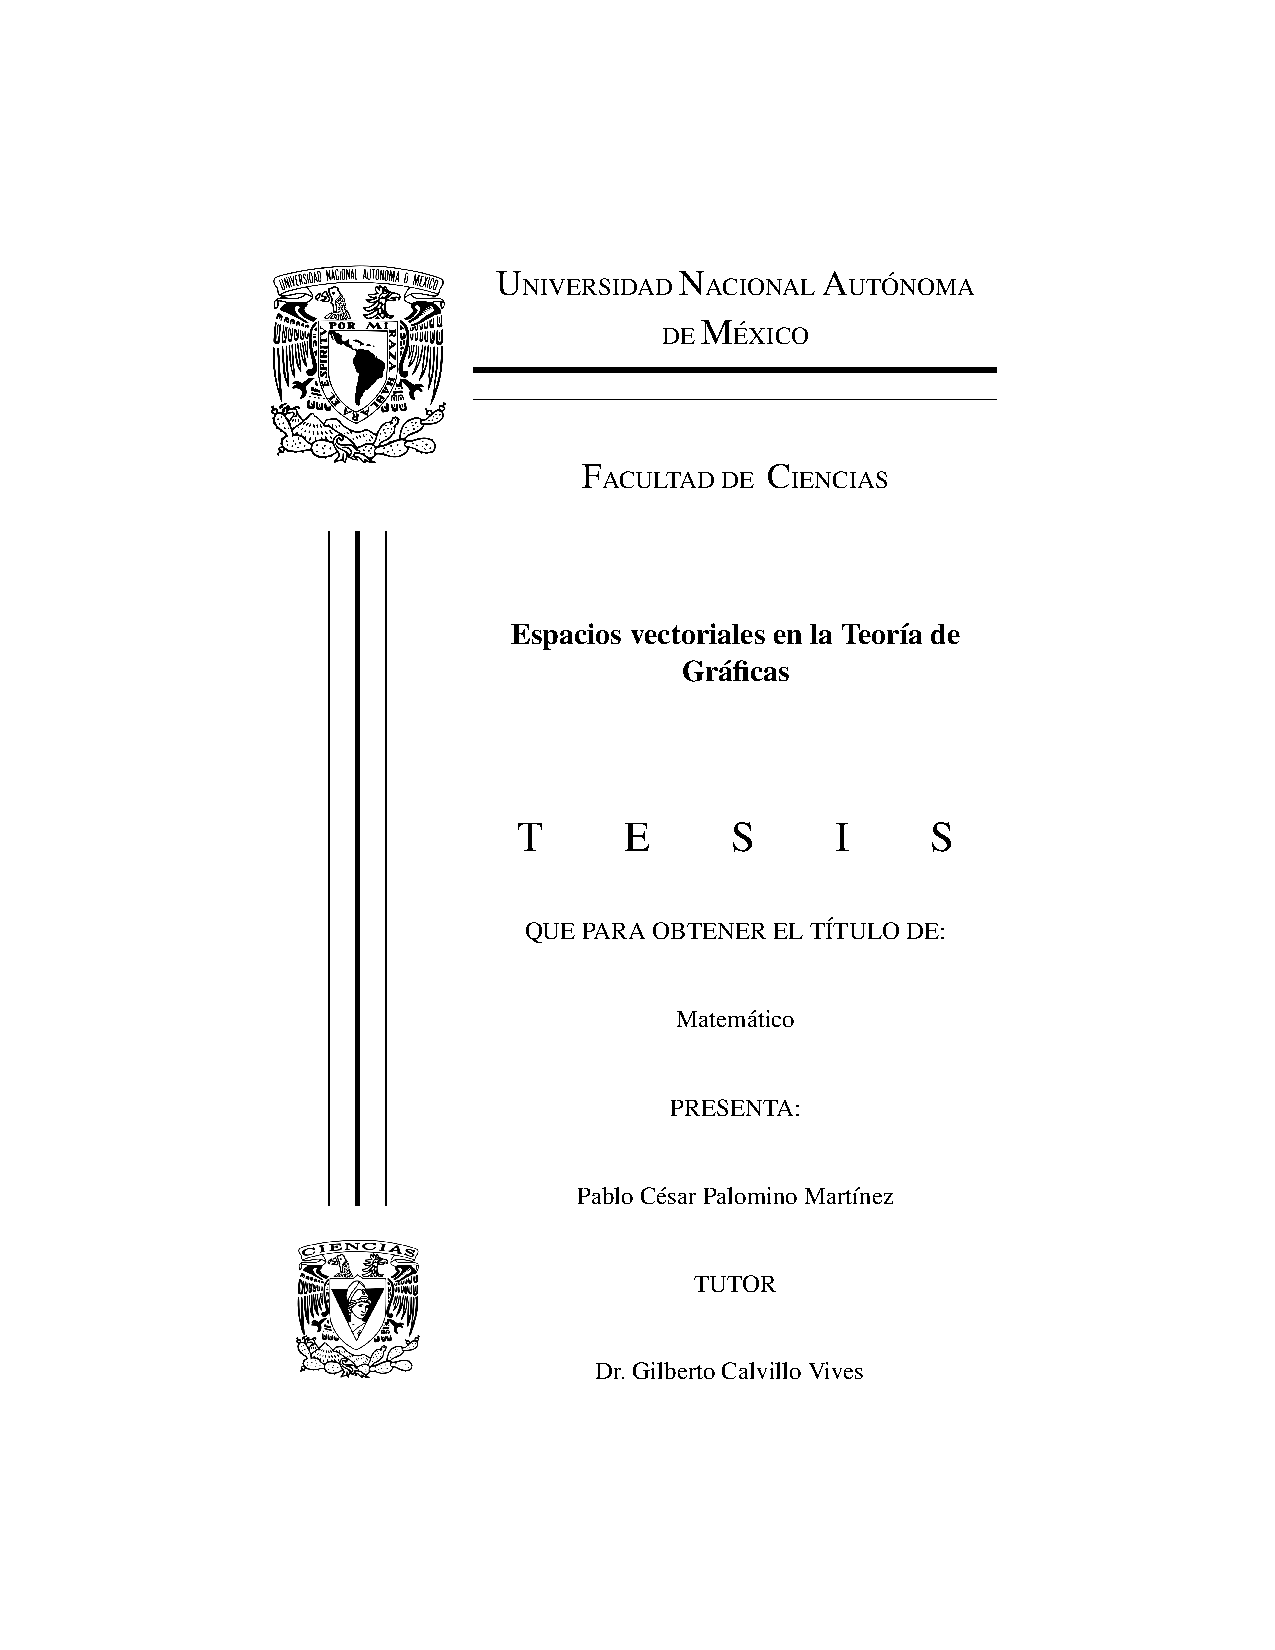
\includepdf[pages=-]{img/PortadaTesis}
           \blankpage{}
           \import{./}{thanks.tex}
            \import{./}{preface.tex}

            \tableofcontents

        \mainmatter %Numeración arábiga
            \import{./}{intro.tex}
            \import{./}{chapter1.tex}
            \import{./}{chapter2.tex}
            \import{./}{chapter3.tex}
            \import{./}{chapter4.tex}

        \printbibliography[heading=bibintoc,title={Bibliografía}]

        \printindex
  
        
    \end{document}
